\documentclass[../ClassicThesis.tex]{subfiles}
\begin{document}

%************************************************
\chapter{Plates}\label{ch:plates}
%************************************************

\section{Overview of approaches for finding plates}

There are multiple approaches for finding plates contained in a 3D~mesh. Two of these concepts, inherent plates \cite[p.~32]{master-thesis} and extrusion \cite[p.~28]{master-thesis}, are based on existing algorithms. The third approach, stacking plates, was built from the ground up.

Inherent plates are modeled in the mesh, with both a top and a bottom side (see Figure \ref{fig:inhplates}). Between these, a plate is constructed. This is the most obvious approach, since it finds plates which a human would identify as well. It is discussed in Section \ref{sec:inherentplates}. The second approach, extruding plates, uses the mesh surface to extrude plates into the object (Figure \ref{fig:extplates}). It is inspired by the extrusion manufacturing process, where a malleable material is pressed through a die. Here, a flat part of the model's surface is translated along its normal, resulting in the opposite side of the plate. This is described further in Section \ref{sec:extrudedplates}. Our algorithm uses a combination of these two concepts. First, the model is searched for inherent plates. Afterwards, all surfaces of the model which were not used for creating a plate yet are forwarded to the extruding algorithm. While the first step finds plates which were actually modeled in the  Thus, we can handle complex meshes which feature both types of plates. 

The concept of stacking plates is described in Section \ref{}

The second approach, extruded plates, uses the mesh surface to extrude plates into the object (Figure \ref{fig:extplates}). While this method works on more meshes then the inherent approach, it can produce doubled plates if they are modeled in the mesh. The third approach is to stack plates, creating a filled approximation of the mesh (Figure \ref{fig:staplates}).

\begin{figure}
    \centering
    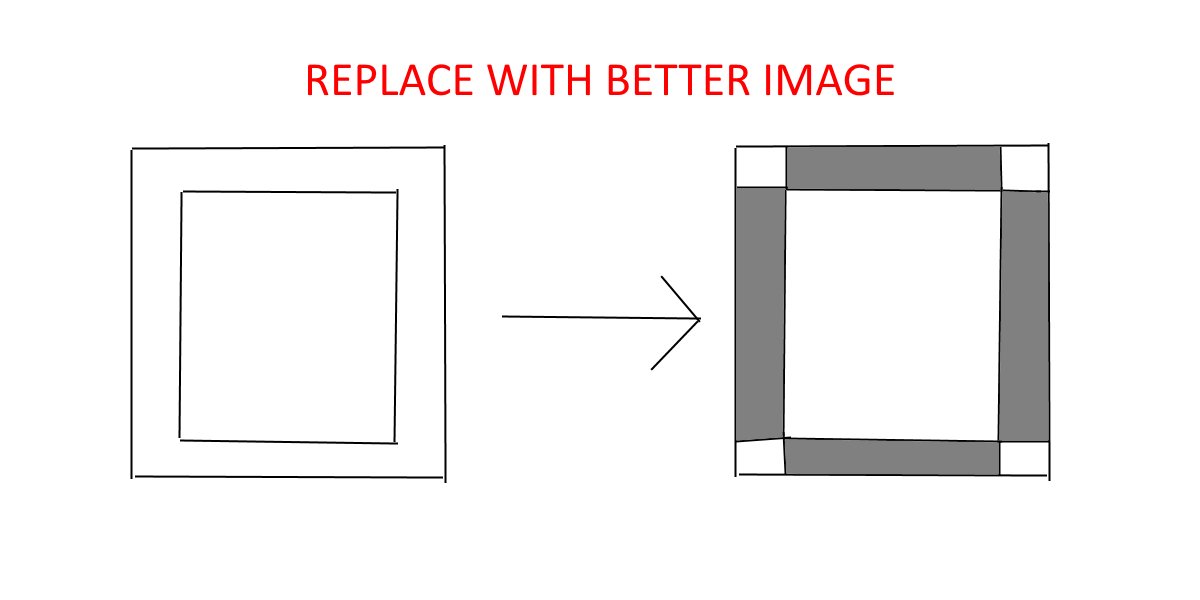
\includegraphics[width=1.0\columnwidth]{Images/plates_inherentplates.png}
    \caption{Finding inherent plates.}
    \label{fig:inhplates}
\end{figure}

\begin{figure}
    \centering
    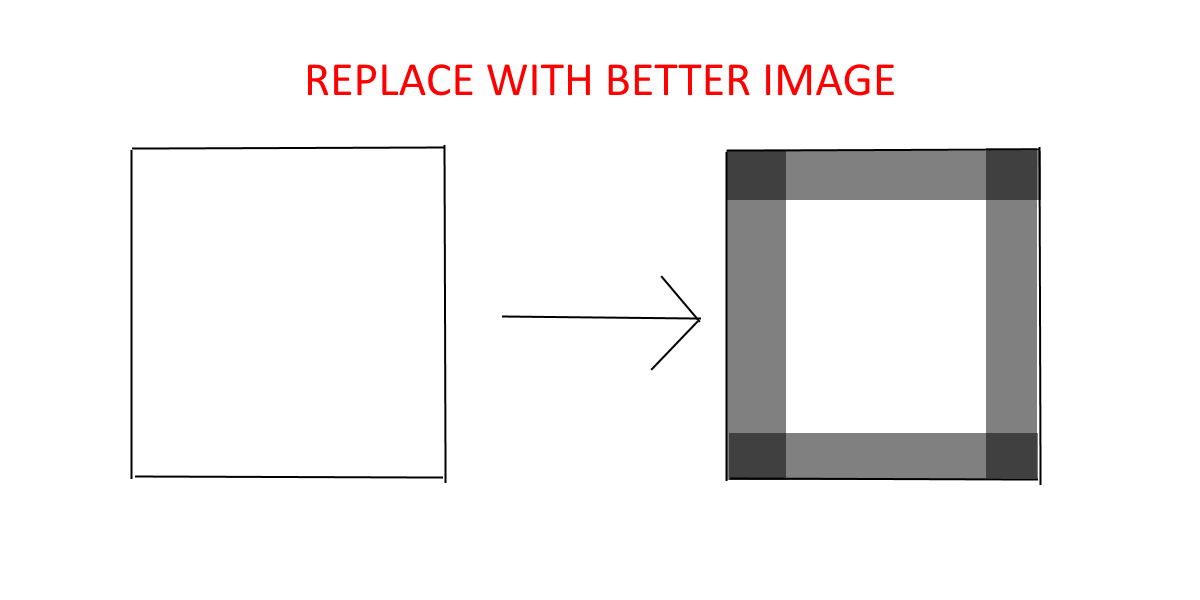
\includegraphics[width=1.0\columnwidth]{Images/plates_extrudedplates.png}
    \caption{Finding extruded plates.}
    \label{fig:extplates}
\end{figure}

\begin{figure}
    \centering
    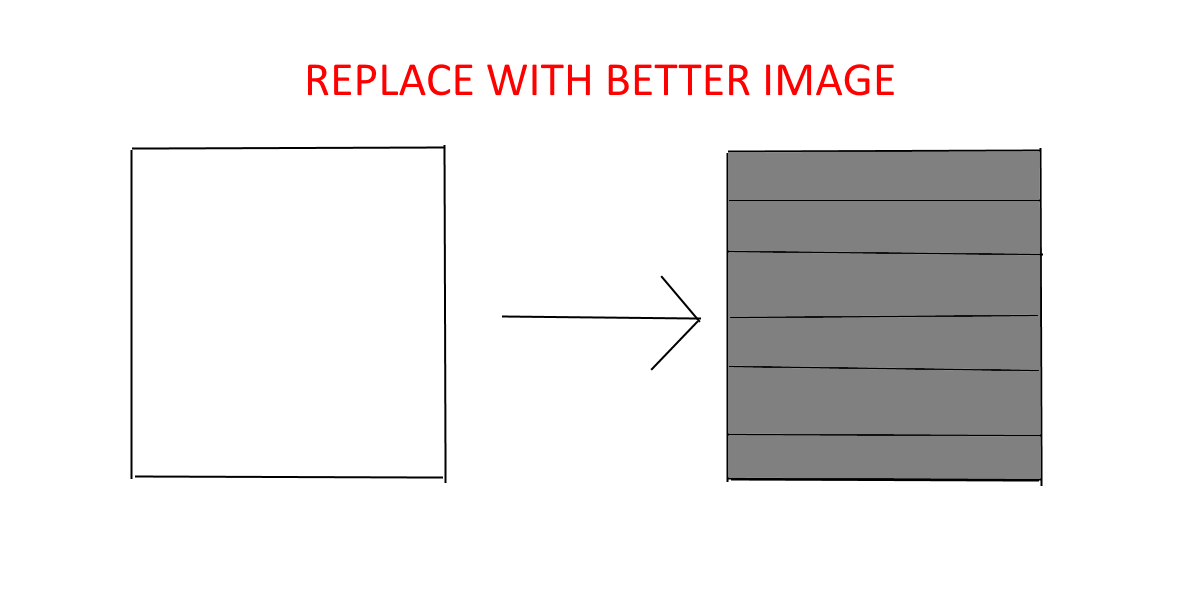
\includegraphics[width=1.0\columnwidth]{Images/plates_stackedplates.png}
    \caption{Finding stacked plates.}
    \label{fig:staplates}
\end{figure}

\section{Prerequisites for finding plates}

Before finding plates, the model's faces have to be grouped into planar surfaces (Figure \ref{fig:coplanar}). This is done by checking the angle between adjacent faces. Afterwards, the resulting shapes' edge loops are generated and the contour is differentiated from the holes.

\begin{figure}
    \centering
    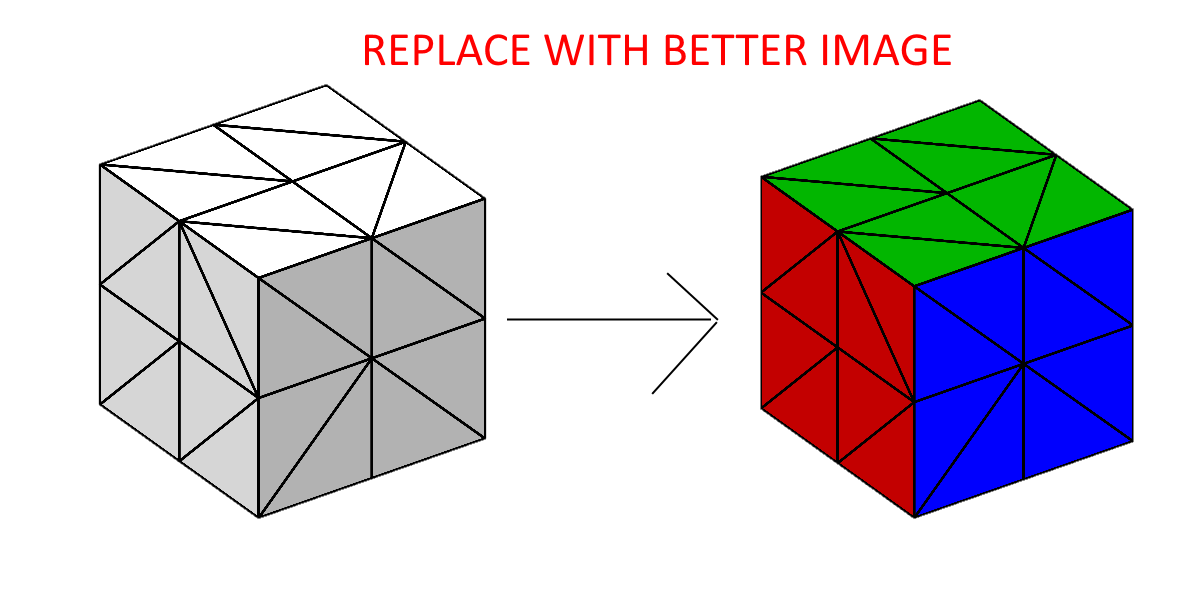
\includegraphics[width=1.0\columnwidth]{Images/plates_coplanar.png}
    \caption{Finding inherent surfaces.}
    \label{fig:coplanar}
\end{figure}

\subsection{Coplanar Faces}

The algorithm for finding coplanar faces requires the models to be stored as a face-vertex mesh. This is calculated by \meshlib, the library used for importing models. In a face-vertex mesh, faces only store their vertices' indices, with the vertices being stored in a different lookup table. This allows for easier adjacency checks - only the vertex indices have to be compared. Additionally, the face normals are stored in an array, in the same order as in the face list.

Now, two more lookup tables are added: One contains all edges (stored as a sorted pair of vertex indices) belonging to each face, while the second one allows looking up the faces adjacent to an edge. Both lists can be created in one single pass (see Listing \ref{lst:lookuptables}). 

\begin{listing}
\begin{minted}[
linenos
]{coffeescript}
setupFaceEdgeEdgeFaceLookup: ->
  for faceIndex in [0...faceCount]
    # Avoid double edges by sorting vertices
    { min_vertex
      mid_vertex
      max_vertex } = @findMinMidMaxVertex()
    # Register which edges this triangle uses.
    @addEntryToEdgeFaceMap(min_vertex, mid_vertex, faceIndex)
    @addEntryToEdgeFaceMap(mid_vertex, max_vertex, faceIndex)
    @addEntryToEdgeFaceMap(min_vertex, max_vertex, faceIndex)
    # Set the edges that make up this triangle.
    @faceVertexMesh.faceToEdges[faceIndex] = [
      [min_vertex, mid_vertex]
      [mid_vertex, max_vertex]
      [min_vertex, max_vertex]
    ]
\end{minted}
\caption{Simplified lookup table generation.}
\label{lst:lookuptables}
\end{listing}

Afterwards, the faces are grouped. This in done by iterating over all faces. When a face is found which has not been visited yet, a new face group is started. Now all of the face's edges are pushed to a queue, along with the current face index (Listing \ref{lst:iteratefaces}).

\begin{listing}
\begin{minted}[
linenos
]{coffeescript}
for faceIndex in [0...faceCount] when not faceVisited[faceIndex]
  faceGroup = [faceIndex]
  faceGroupIndex = faceGroups.length
  outerEdgeGroup = []
  groupNormal = @faceVertexMesh.getFaceNormal(faceIndex)
  @faceToFaceGroup[faceIndex] = faceGroupIndex
  faceVisited[faceIndex] = true
  # connect the adjacent faces
  edgeQueue = []
  adjacentEdges = @faceVertexMesh.getEdgesFromFace(faceIndex)
  for edge in adjacentEdges
    edgeQueue.push({ edge, faceIndex })
  @traverseAdjacentFaces(...)
\end{minted}
\caption{Iteration over faces with creation of new face groups.}
\label{lst:iteratefaces}
\end{listing}

There are multiple important variables being set here: First, we have the new \mintinline{coffeescript}{faceGroup}, containing only the current face. Next, we have the index of the group, used for creating a \mintinline{coffeescript}{faceToFaceGroup} lookup table. The \mintinline{coffeescript}{outerEdgeGroup} contains all edges surrounding the group, which allows the creation of a shape containing the face group. The group's normal vector is initialized with the current face's normal vector. Lastly, the current face is marked as visited in order to avoid checking it multiple times.

After the edges have been pushed in the queue, we start processing it (see Listing \ref{lst:traverseadjacent}).  

\begin{listing}
\begin{minted}[
linenos,breaklines
]{coffeescript}
traverseAdjacentFaces: tco (...) ->
  if edgeQueue.length is 0
    return
  { edge, faceIndex } = edgeQueue.shift()
    faceNormal = @faceVertexMesh.getFaceNormal(faceIndex)
  # get the faces from the edge
  adjacentFaces = @faceVertexMesh.getFacesFromEdge(
    edge[0]
    edge[1]
  )
  continued = false
  for nextFaceIndex in adjacentFaces when nextFaceIndex isnt faceIndex
    # check if faces are coplanar
    # [...]
  if not continued and edge[0] isnt edge[1]
    # the edge is an outer edge for this coplanar group
    outerEdgeGroup.push(edge)
  @recur(...)
\end{minted}
\caption{Function repeated for each edge in queue.}
\label{lst:traverseadjacent}
\end{listing}

\todo{list tco code? or just mention?}

This is implemented as a \emph{tail recursion}, the helper function \mintinline{coffeescript}{tco} is based on an existing implementation of tail calls in \coffeescript\footnote{TCO in \coffeescript, \url{https://gist.github.com/adrusi/1905351}}. It runs \mintinline{coffeescript}{traverseAdjacentFaces} as long as \mintinline{coffeescript}{recur} is called each pass. First, the length of the queue is checked. If there a no more edges waiting to be processed, we can jump out of the recursion and continue searching for new groups (Listing \ref{lst:iteratefaces}). Otherwise, we first get the normal of the face from which we came. Next, we extract the new face from the edge and get the face's normal as well. After checking the faces' coplanarity, we signal that there may be more elements in the queue by calling \mintinline{coffeescript}{recur}.

Listing \ref{lst:coplanarcheck} shows what happens when testing for coplanarity. \mintinline{coffeescript}{isAngleZero} calculates the angle between the normals and compares it to zero. This is done even if the new face was already visited. If the faces are not coplanar, the edge is added to the group's outer edges. In case of coplanarity, we now check if the face was visited. If it was not, it is added to the face group. Additionally, an entry is added to the \mintinline{coffeescript}{faceToFaceGroup} lookup table and the face is marked as visited. After fetching the face's edges, they are pushed into the queue.

\begin{listing}
\begin{minted}[
linenos,breaklines
]{coffeescript}
if @isAngleZero(faceNormal, nextFaceNormal)
  if not faceVisited[nextFaceIndex]
    faceGroup.push(nextFaceIndex)
    groupNormal.add(nextFaceNormal)
    @faceToFaceGroup[nextFaceIndex] = faceGroupIndex
    faceVisited[nextFaceIndex] = true
    adjacentEdges = @faceVertexMesh.getEdgesFromFace(nextFaceIndex)
    for nextEdge in adjacentEdges when not Util.arrayEquals edge, nextEdge
      edgeQueue.push({ edge: nextEdge, faceIndex: nextFaceIndex })
else
  outerEdgeGroup.push(edge)
\end{minted}
\caption{Check for coplanar faces.}
\label{lst:coplanarcheck}
\end{listing}

After all faces have been processed and assigned a group, the \mintinline{coffeescript}{faceGroups}, \mintinline{coffeescript}{faceGroupNormals} and \mintinline{coffeescript}{outerEdgeGroups} are injected into the face-vertex mesh, along with the \mintinline{coffeescript}{faceToFaceGroup} lookup table.

\subsection{Shape Finder / Deus}

\note{TODO}

The shape finder creates shapes from the outer edge loops of the found coplanar faces. The outer edge loop is a set of edges in the format [vertex_index_1, vertex_index_2]. This is converted into a set of continuous edge loops of the form [vertex_index_1, vertex_index_2, ..., vertex_index_n, vertex_index_1]

\subsection{Hole Detection / Dimitri}

PASTE HERE

\section{Finding inherent plates}\label{sec:inherentplates}

In order to find inherent plates in a mesh, the first step is to find all coplanar shapes which are parallel and check if the distance between them fits one of the given plate thicknesses (Listing \ref{lst:platecand}).

\begin{listing}
\begin{minted}[
linenos,breaklines
]{coffeescript}
candidates = []
for shape1, index1 in shapes
  for shape2, index2 in shapes when index1 < index2
    if @normalsParallelAndSurfacesFacingApart shape1, shape2
      thickness = @checkPlateThickness shape1, shape2
        if thickness?
          candidates.push { shape1, shape2, thickness }
return candidates
\end{minted}
\caption{Finding plate candidates.}
\label{lst:platecand}
\end{listing}

\subsection{Checking parallelism}

While the testing for normal parallelism is done with built-in vector functions, the check if the shapes are facing apart uses a vertex of each of the surfaces and calculates the angle of the resulting vector to one of the normals. If this angle is smaller than 90\textdegree, the surfaces are indeed facing apart.

\subsection{Calculating best plate thickness}

The calculation of the optimal plate thickness is shown in Listing \ref{lst:checkplatethickness}. First, the actual distance between the shapes is calculated. Next, all possible plate thicknesses are tested if they can approximate the actual thickness well enough. Lastly, the thickness with the lowest absolute deviation is chosen as the best thickness.

\begin{listing}
\begin{minted}[
linenos,breaklines
]{coffeescript}
checkPlateThickness: (shape1, shape2) ->
  actualThickness = @distanceBetweenPlanes shape1, shape2
  okThicknesses = []
  # check which thicknesses are ok factor-wise
  for plateThickness in @plateThicknesses
    if plateThickness * @minThicknessDeviationFactor < actualThickness < plateThickness * @maxThicknessDeviationFactor
      okThicknesses.push plateThickness
  bestThickness = null
  bestDeviation = null
  for plateThickness in okThicknesses
    deviation = Math.abs(plateThickness - actualThickness)
    if bestDeviation is null or deviation < bestDeviation
      bestDeviation = deviation
      bestThickness = plateThickness
  return bestThickness
\end{minted}
\caption{Finding the best plate thickness.}
\label{lst:checkplatethickness}
\end{listing}

\subsection{Creating plates}

After finding these plate candidates, the shape which plane's distance to the origin (the z-value of all vertices when laid into the x-y-plane) is smaller is selected as the base shape of the plate, as shown in Listing \ref{lst:faceintersect}. Now, the intersection of both shapes is calculated. This is done by using the already calculated mapping of vertices into the x-y-plane. The resulting intersection is transformed back into 3D-space using the rotation matrix of the base shape. With the resulting shapes, plates are created.

\begin{listing}
\begin{minted}[
linenos
]{coffeescript}
shape2CloserToOrigin = abs(shape2.zValue) < abs(shape1.zValue)
polygon1 = create2DPolygon(shape1)
polygon2 = create2DPolygon(shape2)
intersection = polygon1.intersect polygon2
shapes = parseToShapes(intersection)
plates = parseToPlates(shapes)
return plates
\end{minted}
\caption{Face intersection for creating inherent plates.}
\label{lst:faceintersect}
\end{listing}

The intersection between the shapes is done using the \jsclipper library. After parsing them into the library's polygon class, they can be easily clipped, resulting in a list of intersections which can be parsed back into shapes. The plate creation is based on the previously selected base shape. While the calculated intersection is used as the shape of the plate, the thickness is computed by subtracting the base shape's z-value from the other shape's z-value. Additionally, the base shape's z-value is used as plane constant.

\section{Extruding plates}\label{sec:extrudedplates}

The extrusion of plates is a simpler approach, which is shown in Listing \ref{lst:extrude}. The selected plate thickness has to be inverted, due to the plate being extruded against the face's normal direction. The plane constant of the plates base plane is the same as the z-value of the shapes x-y-representation. After checking the shape's area, the new plate is created.

\begin{listing}
\begin{minted}[
linenos
]{coffeescript}
createPlateFromShape: (shape) ->
  thickness = -@plateThicknesses[0]
  planeConstant = shape.edgeLoops[0].xyPlaneVertices[0].z
  if shape.getContour().computeArea() > @areaThreshold
    return new Plate shape, thickness, planeConstant
  else
    return null
\end{minted}
\caption{Extruding a plate from a shape.}
\label{lst:extrude}
\end{listing}

\section{Removing contained plates / Dimitri}

PASTE HERE

\section{Stacking plates}\label{sec:stackedplates}

As an alternative approach, plates can be stacked. This method does not directly use the models surfaces. However, they can be used for optimization.
The main function for stacking is shown in Listing \ref{lst:stackedmain}. First, the model is rotated in order to optimize the stacking direction. Afterwards, the clipping planes are calculated. After clipping the models faces with these planes, the resulting edges are merged into edge loops, which are used for creating shapes and, as wall as helper objects, polygons. With these, shafts can be added, which connect plates for easier assembly. Afterwards, plates are created. These have to be rotated back based on the original rotation in order to align them with the model. 

\begin{listing}
\begin{minted}[
linenos
]{coffeescript}
findStackedPlates: (model, shapes) ->
  return new Promise (resolve) =>
    rotationMatrix = @findRotation shapes
    model.getClone().then((clone) =>
      @model = @rotateModel clone, rotationMatrix
      @planes = @getClippingPlanes()
      @clipFacesAgainstPlanes @model.model.mesh.faces
      @mergeEdgesInPlanes()
      @shapeGroups = @createShapes()
      @polygonGroups = @createPolygons()
      @shafts = @findShafts()
      @shapes = @clipShafts()
      plates = @createPlates().filter((p) -> p?)
      shaftPlates = @createShaftPlates()
      plates = plates.concat shaftPlates
      plates = @rotatePlatesBack plates, rotationMatrix
      resolve plates
    )
\end{minted}
\caption{Plate stacking main function.}
\label{lst:stackedmain}
\end{listing}

\subsection{Rotating the model}

In order to find a good rotation, the model's biggest surface is aligned to the x-y-plane. While the approach of stacking plates doesn't require information about the model's coplanar surfaces, this optimization does. By iteration over them, the biggest surface's rotation matrix can be found (see Listing \ref{lst:findrotation}). This matrix can be used for transforming all vertices so that the chosen surface is parallel to the x-y-plane.

\begin{listing}
\begin{minted}[
linenos
]{coffeescript}
findRotation: (shapes) ->
  maxArea = 0
  rotationMatrix = new THREE.Matrix3()
  shapes.forEach((shape) ->
    area = shape.area || shape.getContour().computeArea()
    if area > maxArea
      maxArea = area
      rotationMatrix = shape.rotationMatrix
  )
  return rotationMatrix
\end{minted}
\caption{Finding an optimal rotation.}
\label{lst:findrotation}
\end{listing}

\subsection{Finding the clipping planes}

Due to the model being rotated, it can be sliced using planes parallel to the x-y-plane. In order to calculate these, the model's bounding box is calculated first. Using the minimal and maximal z-value, planes are creates with an distance equal to the selected plate thickness. These planes are constructed from a \threejs plane object and a (initially empty) list of edges located in this plane. The planes are displaced by half the plate thickness. Thus, the sampling happens in the middle of the plates-to-be, which is an approximation which works for most applications. The plane creation is shown in Listing \ref{lst:clippingplanes}.

\begin{listing}
\begin{minted}[
linenos,breaklines
]{coffeescript}
getClippingPlanes: ->
  planes = []
  for i in [@minZ..@maxZ] by @thickness
    planes.push {
      plane: new THREE.Plane(
        new THREE.Vector3(0, 0, 1), 
        -(i + @thickness / 2)
      )
      edges: []
    }
  return planes
\end{minted}
\caption{Clipping plane generation.}
\label{lst:clippingplanes}
\end{listing}

\subsection{Clipping the model's faces}

Clipping each face with each plane would be very slow. Thus, we first find one plane which clips the face and check the adjacent planes afterwards (see Listing \ref{lst:clipfaceplanes}). I order to quickly find this plane, binary search is used, as shown in Listing \ref{lst:findplane}. Starting at the median plane (\mintinline{coffeescript}{@planes.length // 2}), we search the planes until one plane clipping the face is found or it is certain that no plane clips the face.

\begin{listing}
\begin{minted}[
linenos
]{coffeescript}
clipFaceAgainstPlanes: (face) ->
  planeIndex = @findClippingPlane(face)
  if planeIndex > -1
    @checkAdjacentPlanes(face, planeIndex)
\end{minted}
\caption{Clipping a face against all planes.}
\label{lst:clipfaceplanes}
\end{listing}

\begin{listing}
\begin{minted}[
linenos,breaklines
]{coffeescript}
findClippingPlane: (face) ->
  stepWidth = @planes.length / 4.0
  index = -1
  currentIndex = @planes.length // 2
  oldIndex = -1
  while currentIndex isnt oldIndex and 0 <= currentIndex < @planes.length and index is -1
    direction = @clipFaceAgainstPlane(
      face, 
      @planes[currentIndex]
    )
    # found clipping plane
    if direction is 0
      index = currentIndex
    # continue search
    else
      oldIndex = currentIndex
      currentIndex += Math.round stepWidth * direction
      stepWidth /= 2
  return index
\end{minted}
\caption{Finding a plane which clips the face.}
\label{lst:findplane}
\end{listing}

The search direction is calculated by clipping the face against the plane (Listing \ref{lst:clipfaceplane}). After clipping each edge with the face, the number of intersection decides the result.

\begin{itemize}
  \item No intersections: The face does not clip the plane.
  \item One Intersection: Invalid. It is not possible to get only one intersection when clipping a valid face.
  \item Two intersections: If both intersection points are the same, one vertex of the face clips the plane. Otherwise two edges clip the plane.
  \item Three intersections: If any two of the intersection points are the same, a vertex and the opposite edge clip the plane. Otherwise the whole face lies in the plane.
\end{itemize}

If the face doesn't clip the plane or only intersect with one vertex, we check if it is below or above the plane and return either -1 or 1 as direction (calculation shown in Listing \ref{lst:facedirection}). In all other cases, 0 is returned, because the face clips the plane and we don't have to search further. 

Additionally, if either two edges, an edge and a vertex or the whole face clips the plane, these intersections are stored in the plane.

\begin{listing}
\begin{minted}[
linenos
]{coffeescript}
clipFaceAgainstPlane: (face, plane) ->
  intersections = []
  face.vertices.forEach((vertex, index) =>
    start = vector(vertex)
    end = vector(face.vertices[(index + 1) % 3])
    line = new THREE.Line3(start, end)
    intersection = plane.plane.intersectLine line
    if intersection? then intersections.push intersection
  )
  # handle intersections
  # [...]
  return direction
\end{minted}
\caption{Clipping a face against a plane.}
\label{lst:clipfaceplane}
\end{listing}

\begin{listing}
\begin{minted}[
linenos
]{coffeescript}
getDirectionFromPlaneToFace: (face, plane) ->
  sum = 0
  face.vertices.forEach((vertex) ->
    sum += vertex.z + plane.plane.constant
  )
  if sum is 0 then throw new Exception()
  return sum / Math.abs sum
\end{minted}
\caption{Calculating the direction from a plane to a face.}
\label{lst:facedirection}
\end{listing}

After one clipping plane has been found, the adjacent ones have to be checked as well, since a face can span over multiple planes. This is done by iterating over the planes, starting from the next one and moving away. If the returned direction is not 0, we can stop because the plane and all following ones do not clip the face. Both directions, upwards and downwards, are checked seperately (see Listing \ref{lst:checkadjacent}).

\begin{listing}
\begin{minted}[
linenos,breaklines
]{coffeescript}
checkAdjacentPlanes: (face, index) ->
  runIndex = index + 1
  direction = 0
  while(runIndex < @planes.length and direction is 0)
    direction = @clipFaceAgainstPlane(
      face, 
      @planes[runIndex++]
    )
  runIndex = index - 1
  direction = 0
  while(runIndex >= 0 and direction is 0)
    direction = @clipFaceAgainstPlane(
      face, 
      @planes[runIndex--]
    )
  return
\end{minted}
\caption{Checking if adjacent planes are clipping too.}
\label{lst:checkadjacent}
\end{listing}

\subsection{Creating shapes}

Using the intersections stored in each plane, shapes can be created. These shapes represent the cross-sections of the model. Since this requires merging the intersection edges, the shapes finder can be re-used for this step. Additionally, the \jsclipper library is used to create 2D polygons, which are used in the next step.

\subsection{Adding shafts}

In order to assemble the stacked plates, we connect them with shafts (Figure \ref{fig:shafts}). Our approach for this: if two shapes which are located in adjacent planes intersect, they have to be connected by at least one shaft. The shaft finding algorithm has three steps: First, we iterate over all shapes and connect as many as possible. Next, we fix shapes which are not yet connected. Afterwards, we clean up shafts which are only connected to one shape.

\begin{figure}
    \centering
    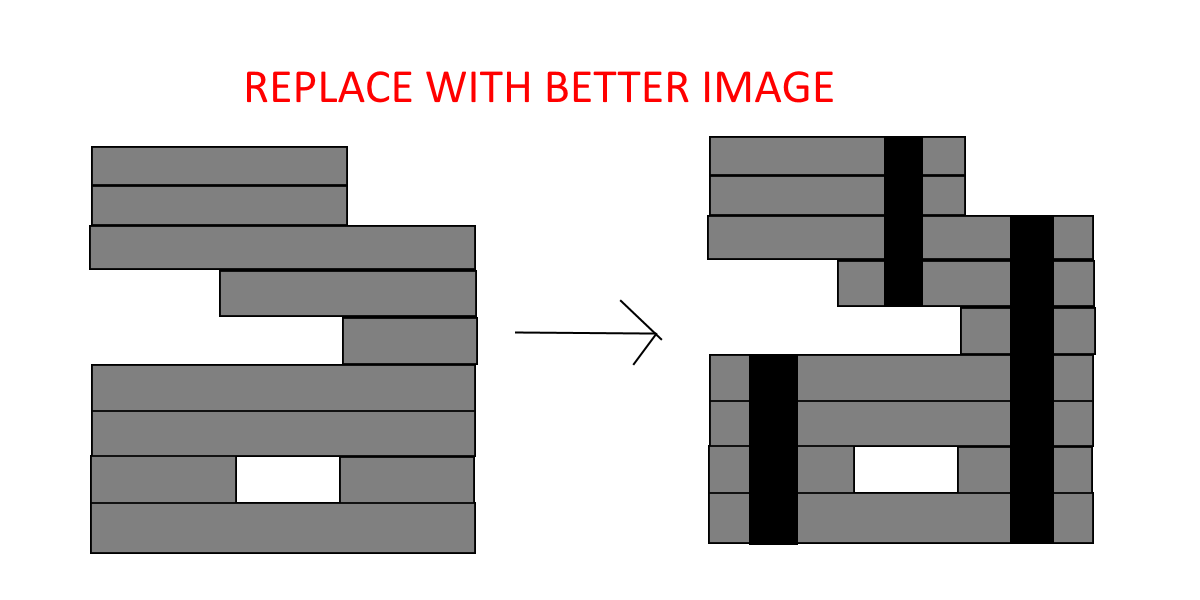
\includegraphics[width=1.0\columnwidth]{Images/plates_shafts.png}
    \caption{Connecting plates with shafts.}
    \label{fig:shafts}
\end{figure}

\subsubsection{The shaft object}

A shaft has these properties:
\begin{itemize}
    \item polygons - a list of the polygons which the shaft connects
    \item intersection - the intersection of all the polygon which the shaft connects
    \item finished - true if the shaft is complete and won't be extended to connect more polygons
    \item lastlevel - the layer of the last added polygon
    \item shaftData - contains the shaft's cross section's x and y dimensions
\end{itemize}
It contains functions which allow adding new polygons to the shaft, and building the shaft's cross section and contour.

\subsubsection{First pass}

Instead of the actual shapes, the corresponding polygons are used, which enable working with the \jsclipper. These are organized in layers, matching the clipping planes. Each layer contains a list of polygons, since there can be multiple shapes in one layer. We have to iterate over both lists, the inner and the outer, as shown in Listing \ref{lst:findshafts}.

When processing a new polygon, we first mark that it has not been added to any shaft yet. Now, we iterate over all shaft candidates. If the current level (the layer) is bigger than the shaft's last added polygon's level plus one, there was no polygon from the last layer added to the shaft. Since we do not want shafts to create "bridges" spanning between unconnected layers, the shaft is marked as completed. If that is not he case, we try to add the polygon to the shaft.

\begin{listing}
\begin{minted}[
linenos,breaklines
]{coffeescript}
findShafts: ->
  shaftCandidates = []
  @polygonGroups.forEach((polygonGroup, level) =>
    polygonGroup.forEach((polygon) =>
      added = false
      shaftCandidates.forEach((shaftCandidate) =>
        if level > shaftCandidate.lastlevel + 1
          shaftCandidate.finished = true
        if not shaftCandidate.finished
          if @tryAddingPolygonToShaftCandidate(
                polygon, shaftCandidate
              )
            shaftCandidate.lastlevel = level
            added = true
      )
      if not added
        if Shaft.isIntersectionBigEnoughForShaft(
              polygon.polygon, @shaftData
            )
          newShaftCandidate = Shaft.fromPolygon(
            polygon,
            level,
            @shaftData
          )
          newShaftCandidate.polygons[0].shafts.push(
            newShaftCandidate
          )
          @tryOverlappingShaftBackwards newShaftCandidate
          shaftCandidates.push newShaftCandidate
    )
  )
  @fixUnconnectedPlates shaftCandidates
  @cleanUpShafts shaftCandidates
  shaftCandidates.forEach((shaft) ->
    shaft.createShaftContourAndCrossSection()
  )
  return shaftCandidates
\end{minted}
\caption{Finding shafts.}
\label{lst:findshafts}
\end{listing}

Listing \ref{lst:addpolytoshaft} shows the calculations run when adding a polygon to a shaft. First, the shaft's intersection and the new polygon are intersected. The resulting intersection is checked if it is big enough to fit the shaft. If that is the case, the shaft's intersection is updated and the polygon is added to the shaft.

\begin{listing}
\begin{minted}[
linenos,breaklines
]{coffeescript}
tryAddingPolygonToShaftCandidate: (
    polygon, shaftCandidate, direction
  ) ->
    clip = polygon.polygon.intersect shaftCandidate.intersection
    if clip.length > 0 and
        Shaft.isIntersectionBigEnoughForShaft clip[0], @shaftData
      newIntersection =
        new jsclipper.Polygon clip[0].getShape(), clip[0].getHoles()
      shaftCandidate.intersection = newIntersection
      if direction is "DOWN" then shaftCandidate.polygons.unshift polygon
      else shaftCandidate.polygons.push polygon
      polygon.shafts.push shaftCandidate
      return true
    return false # no intersection
\end{minted}
\caption{Adding a polygon to a shaft.}
\label{lst:addpolytoshaft}
\end{listing}

If the polygon can not be added to any of the shafts, we create a new one - if the polygon is big enough (Listing \ref{lst:findshafts}). Additionally, the shaft is overlapped "backwards", up to three layers. This improves stability in the assembled model.

\subsubsection{Fixing unconnected plates}

In some cases, not all polygons - and thus not all plates - are connected to the others yet. Additionally, shafts should be expanded in both directions as far as possible. A fix is shown in Listing \ref{lst:fixunconnected}.

Each polygon is checked how well it is connected to other polygons. If it is connected to both a polygon below and above (\mintinline{coffeescript}{connection.isConnected} is true), we do not have to connect it further. Otherwise, the shafts connecting it from above and below are checked. We try to expand these to connect more polygons in the given direction. If this succeeds, handling for this polygon is completed. Otherwise, we create a new shaft at this polygon and try to expand it in both directions.

\begin{listing}
\begin{minted}[
linenos,breaklines
]{coffeescript}
fixUnconnectedPlates: (shaftCandidates) ->
  @polygonGroups.forEach((polygonGroup, level) =>
    polygonGroup.forEach((polygon) =>
      connection = @isPolygonConnected polygon, level
      if not connection.isConnected
        expanded = false
        direction = "DOWN"
        if connection.shaftsFromAbove.length > 0
        expanded = @tryExpandingShaftsInOneDirection(
          connection.shaftsFromAbove, level, direction
        )
        if connection.shaftsFromBelow.length > 0
          direction = "UP"
          expanded = @tryExpandingShaftsInOneDirection(
            connection.shaftsFromBelow, level, direction
          )
        if not expanded and 
            Shaft.isIntersectionBigEnoughForShaft(
              polygon.polygon, @shaftData
            )
          newShaftCandidate = Shaft.fromPolygon(
            polygon
            level
            @shaftData
          )
          newShaftCandidate.polygons[0].shafts.push(
            newShaftCandidate
          )
          @tryExpandingShaftAroundLevel(
            newShaftCandidate
            level
            direction
          )
          shaftCandidates.push newShaftCandidate
    )
  )
\end{minted}
\caption{Fixing unconnected plates.}
\label{lst:fixunconnected}
\end{listing}

\subsubsection{Cleaning up shafts}

As a result of this method, polygons which are not adjacent to any other polygon get assigned an own shaft. Since this does not improve the models stability, these are removed again, as shown in Listing \ref{lst:cleanupshafts}.

\begin{listing}
\begin{minted}[
linenos
]{coffeescript}
cleanUpShafts: (shafts) ->
  if shafts.length > 0
    for i in [shafts.length - 1..0]
      if shafts[i].polygons.length < 1
        log.error "FOUND SHAFT WITH ZERO POLYGONS"
      if shafts[i].polygons.length < 2
        shafts[i].polygons.forEach((polygon) ->
          polygon.shafts.splice polygon.shafts.indexOf(shafts[i]), 1
        )
        shafts.splice i, 1
\end{minted}
\caption{Cleaning up shafts.}
\label{lst:cleanupshafts}
\end{listing}

\subsection{Creating plates}

After the shafts are found, their cross section is cut from the connected polygons. Next, these polygons are parsed into shapes and plates. Additionally, the shafts' contours are calculated, with additional plates being created from them. Together, all plates are returned.

\end{document}